\section{Introduction}
The goal of the project work was to implement a peripheral driver for the STM32f407 microcontroller. The implemented driver enables the use of the analog-to-digital converter (ADC). The microcontroller which contains the analog-to-digital converter is located on a development board (STM32 F4 Discovery kit) shown in figure \ref{fig:Board}. This development board contains components that can be interfaced with the microcontroller.\\

\begin{figure}[htbp]
  \centering
     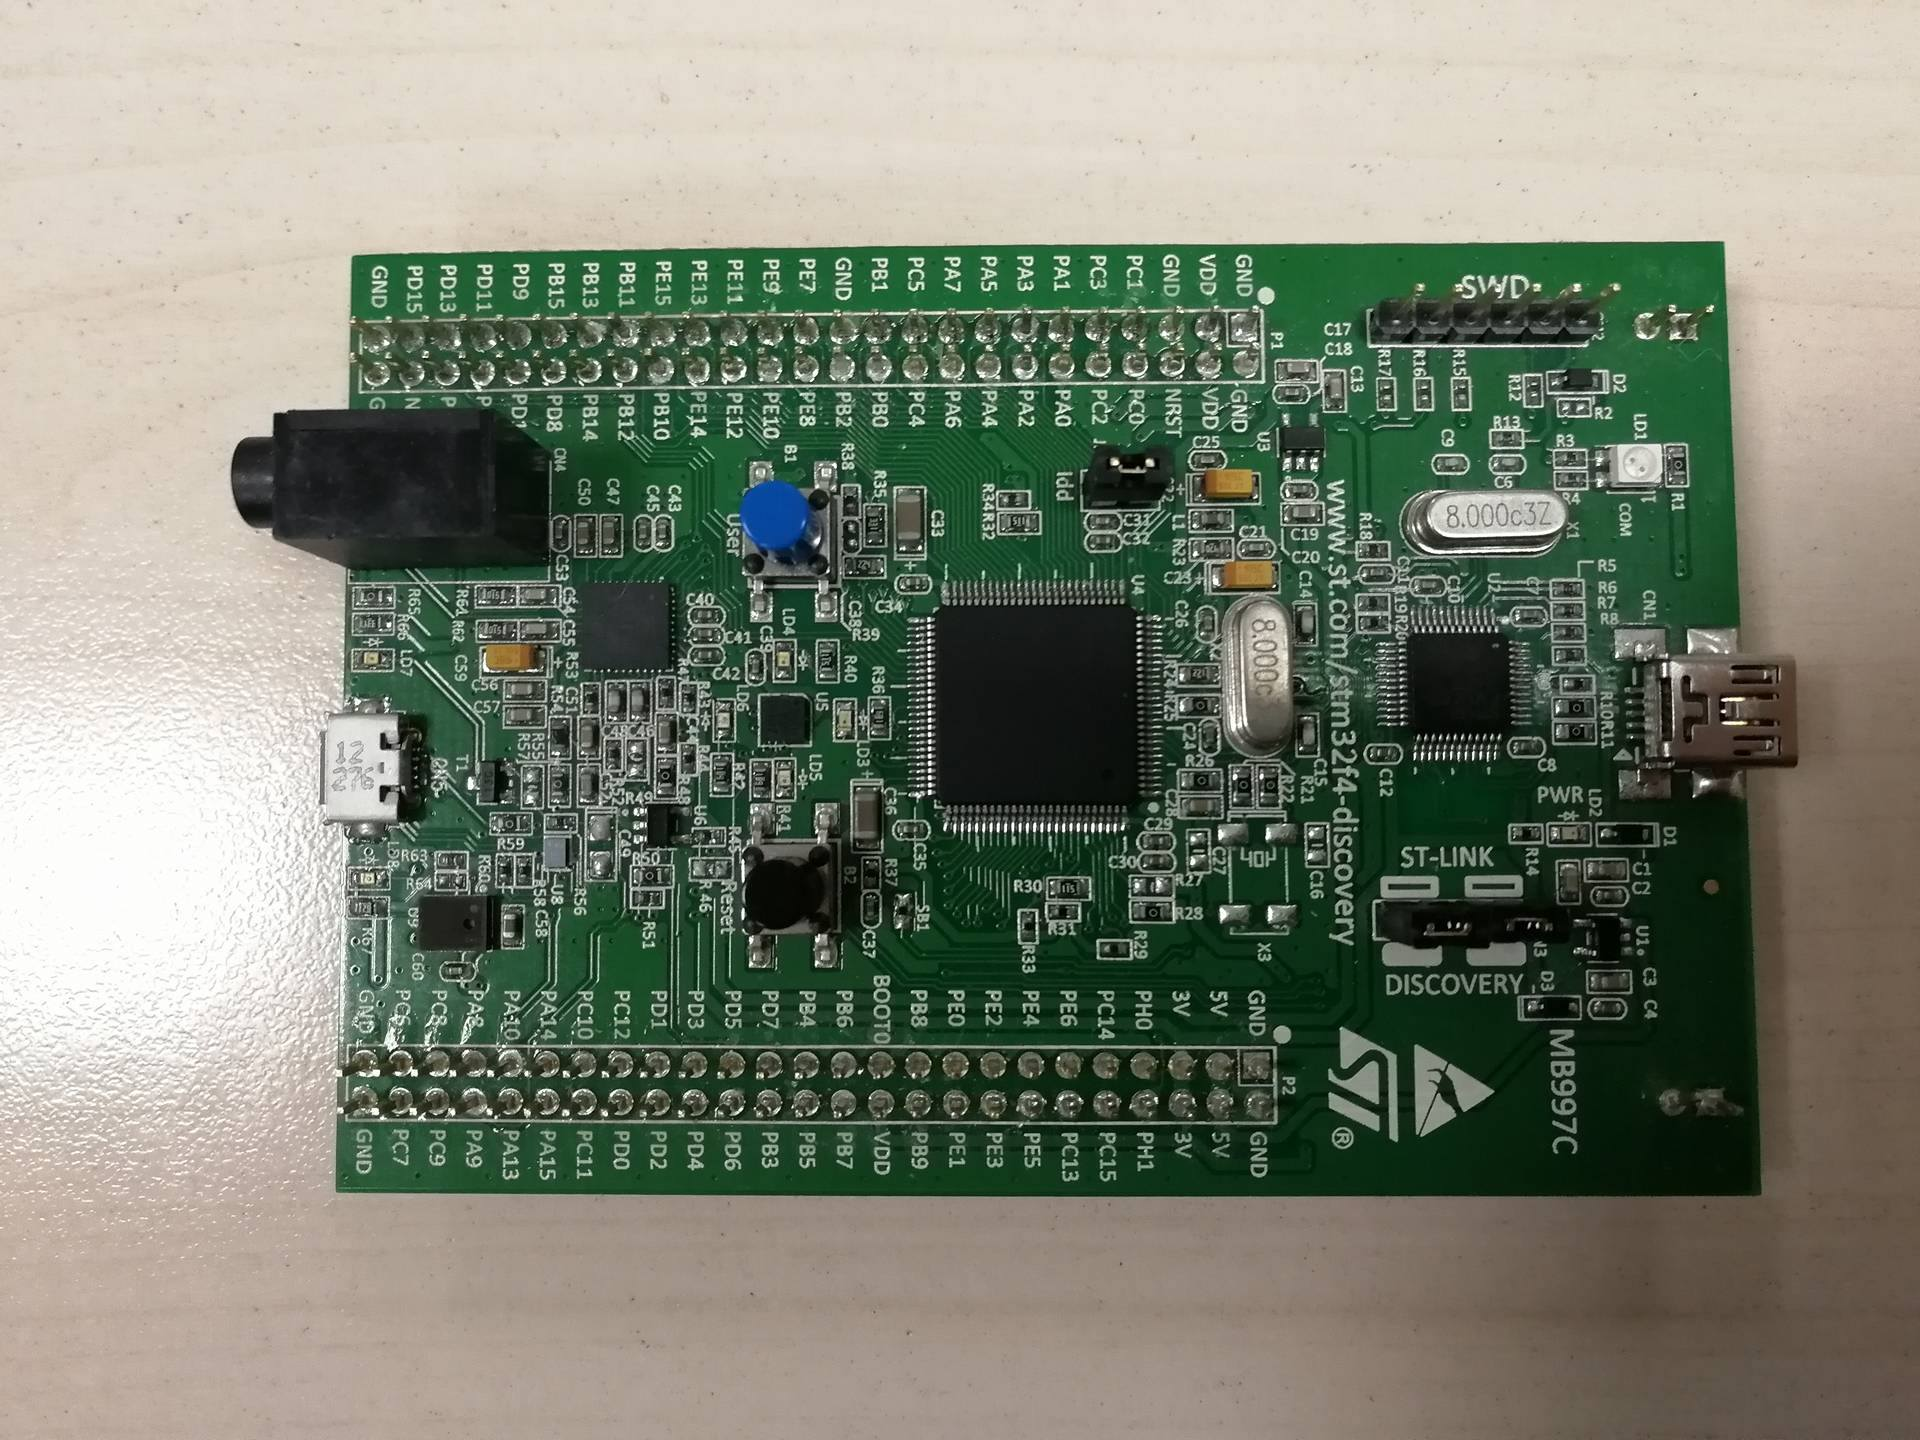
\includegraphics[width=0.7\textwidth]{./figures/board.jpg}
  \caption{Discovery Board}
  \label{fig:Board}
\end{figure}

\begin{figure}[htbp]
  \centering
     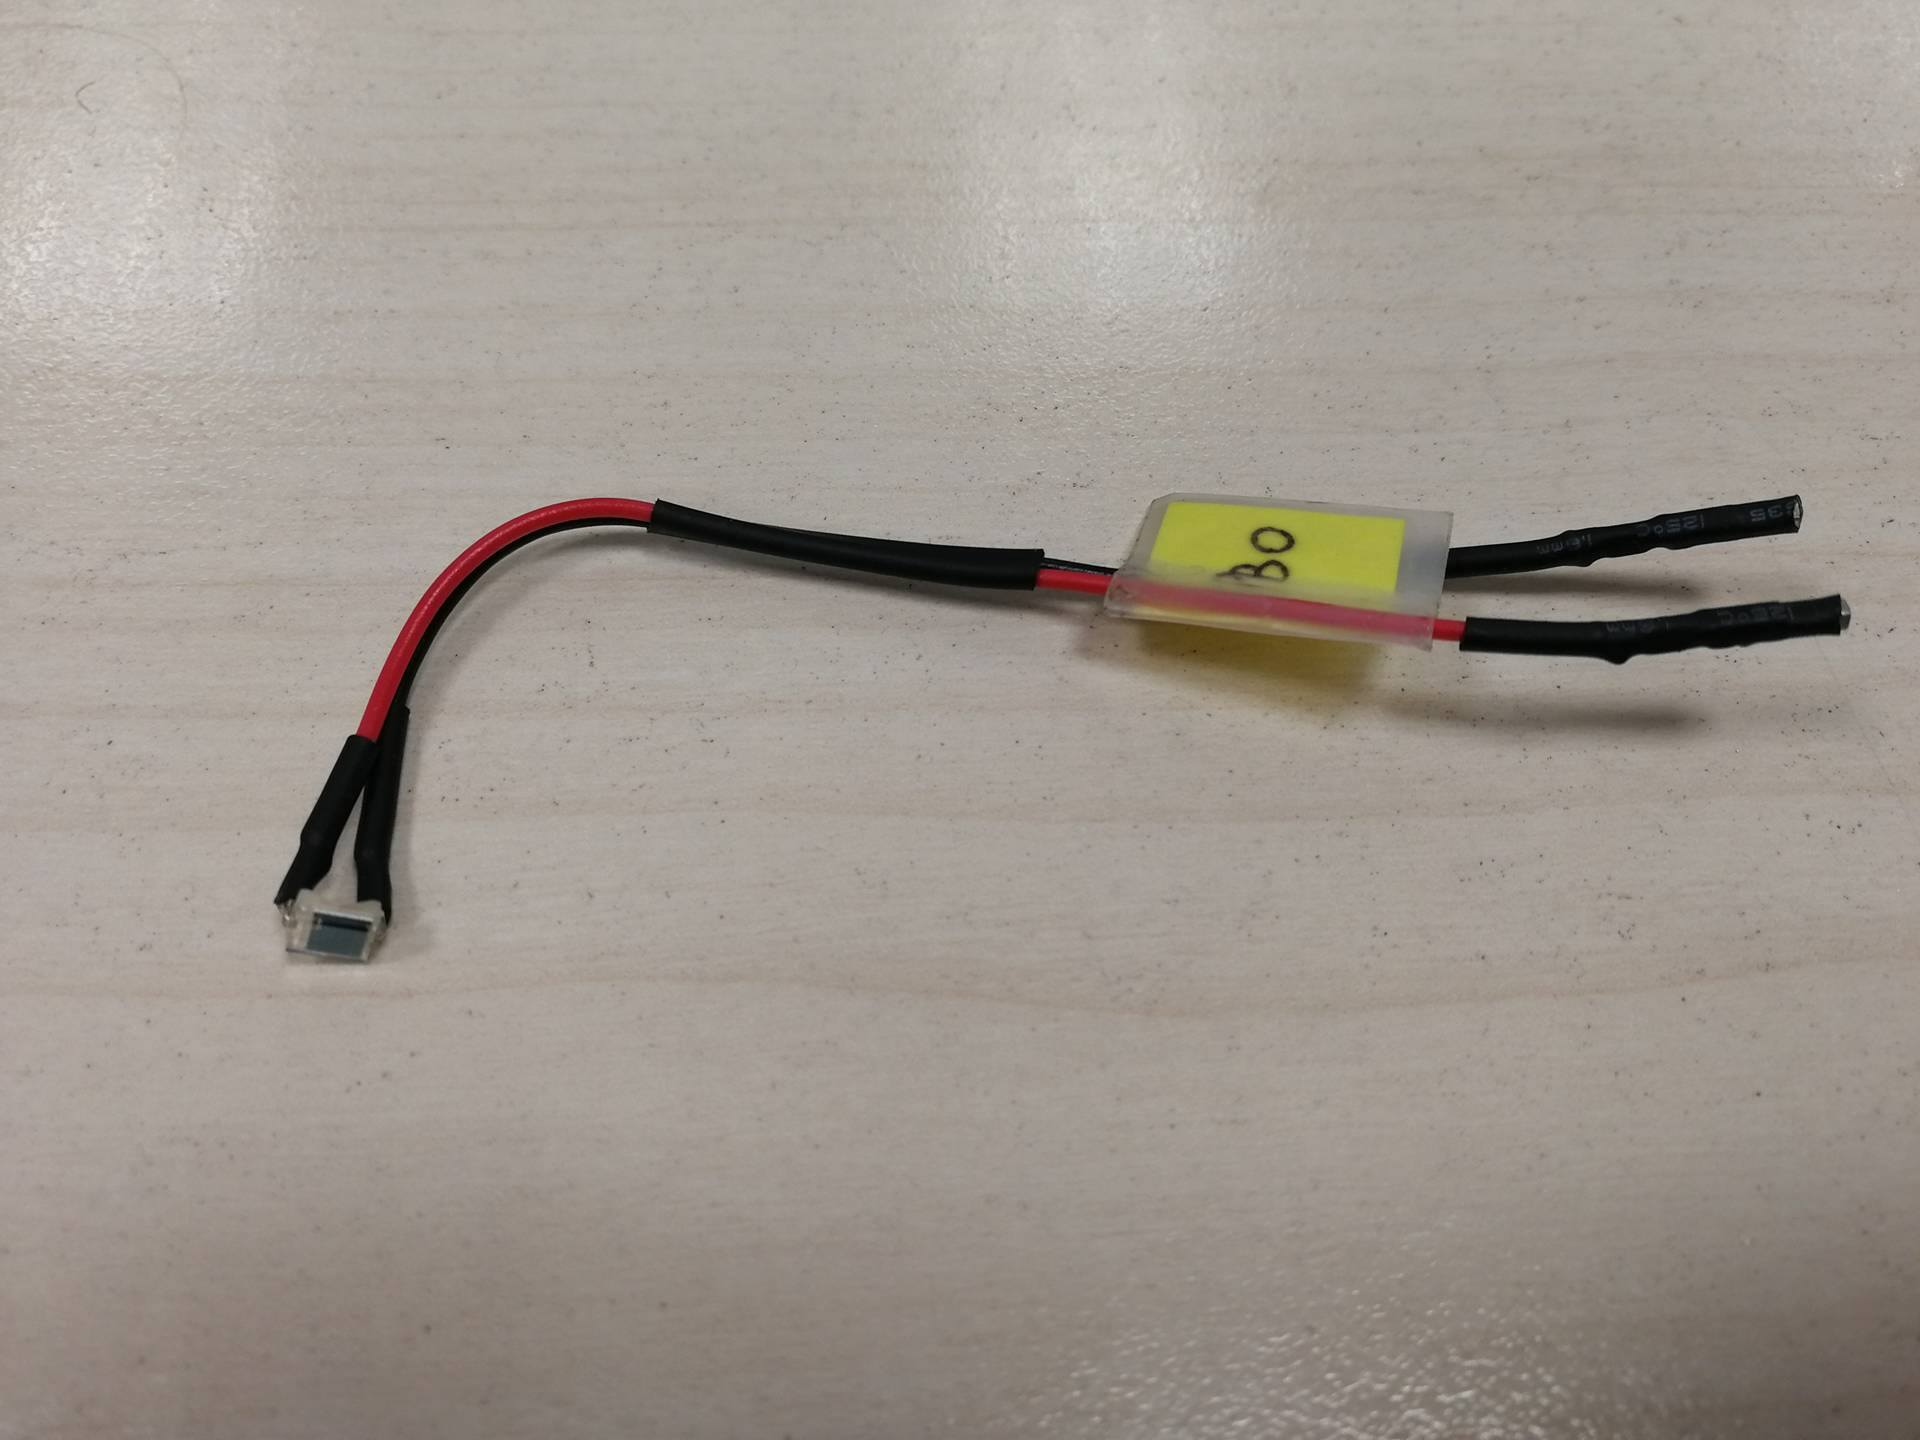
\includegraphics[width=0.5\textwidth]{./figures/photodiode.jpg}
  \caption{Photodiode}
  \label{fig:photodiode}
\end{figure}

\par
In this work the push buttons and LEDs were utilized. An external photodiode shown in figure \ref{fig:photodiode} was connected to the development board connection pins. These components were used to make a simple user reaction game.

\pagebreak


\section{Design and implementation}
\subsection{Game logic}
The idea of the implemented game was to test the reaction time of a player. This game can be played by a defined number of players. The reaction time of a player is evaluated by indicating a start signal and after this signal the player has to cover the photodiode as fast as possible. The game logic is illustrated in figure \ref{fig:GameLogicDiagram}. 

\begin{figure}[htbp]
  \centering
     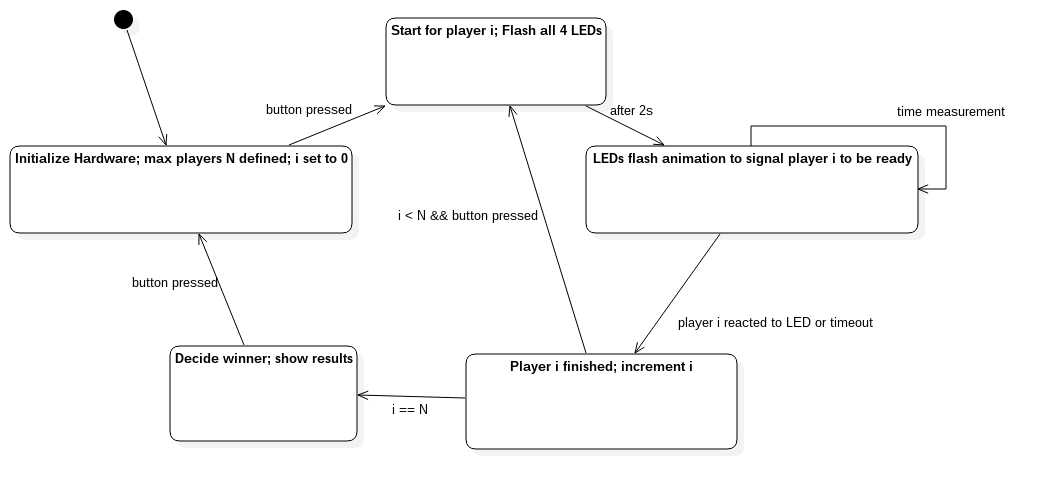
\includegraphics[width=1\textwidth]{./figures/FSM_Diagram.png}
  \caption{Game logic diagram}
  \label{fig:GameLogicDiagram}
\end{figure}

As illustrated in figure \ref{fig:GameLogicDiagram} the game is started after the hardware initialization has been completed. This is done when the power of the board is turned on and the board's push button has been pressed. Information about the game status and corresponding instructions are printed on a serial monitor. These instructions are shown in chapter \ref{Results}.\\
\par
After the push button has been pressed it is the first player's turn and all of the user programmable LEDs start to flash rapidly for a short duration and then turn off. This is an indication to the player to get ready to get ready. After this the LEDs start to light up in a clockwise orientation one by one. Once the fourth LED has lighten up, the player has to cover the photodiode as quickly as possible. Player reaction time is measured from the fourth LED lighting up and to the point when the photodiode has been covered.\\ 
\par
Then another player starts their turn by pressing the push button and has to interact in the same manner as the player before. This cycle is repeated until all of the players have had their turn. The reaction times are finally displayed and the player who had the lowest reaction time wins the game. A new game can be started by pressing the push button.

\subsection{Peripheral drivers}
%ADC
%Push button
%LED
%Serial
%timer
%connections
\cite{RefManual}
\begin{figure}[htbp]
  \centering
     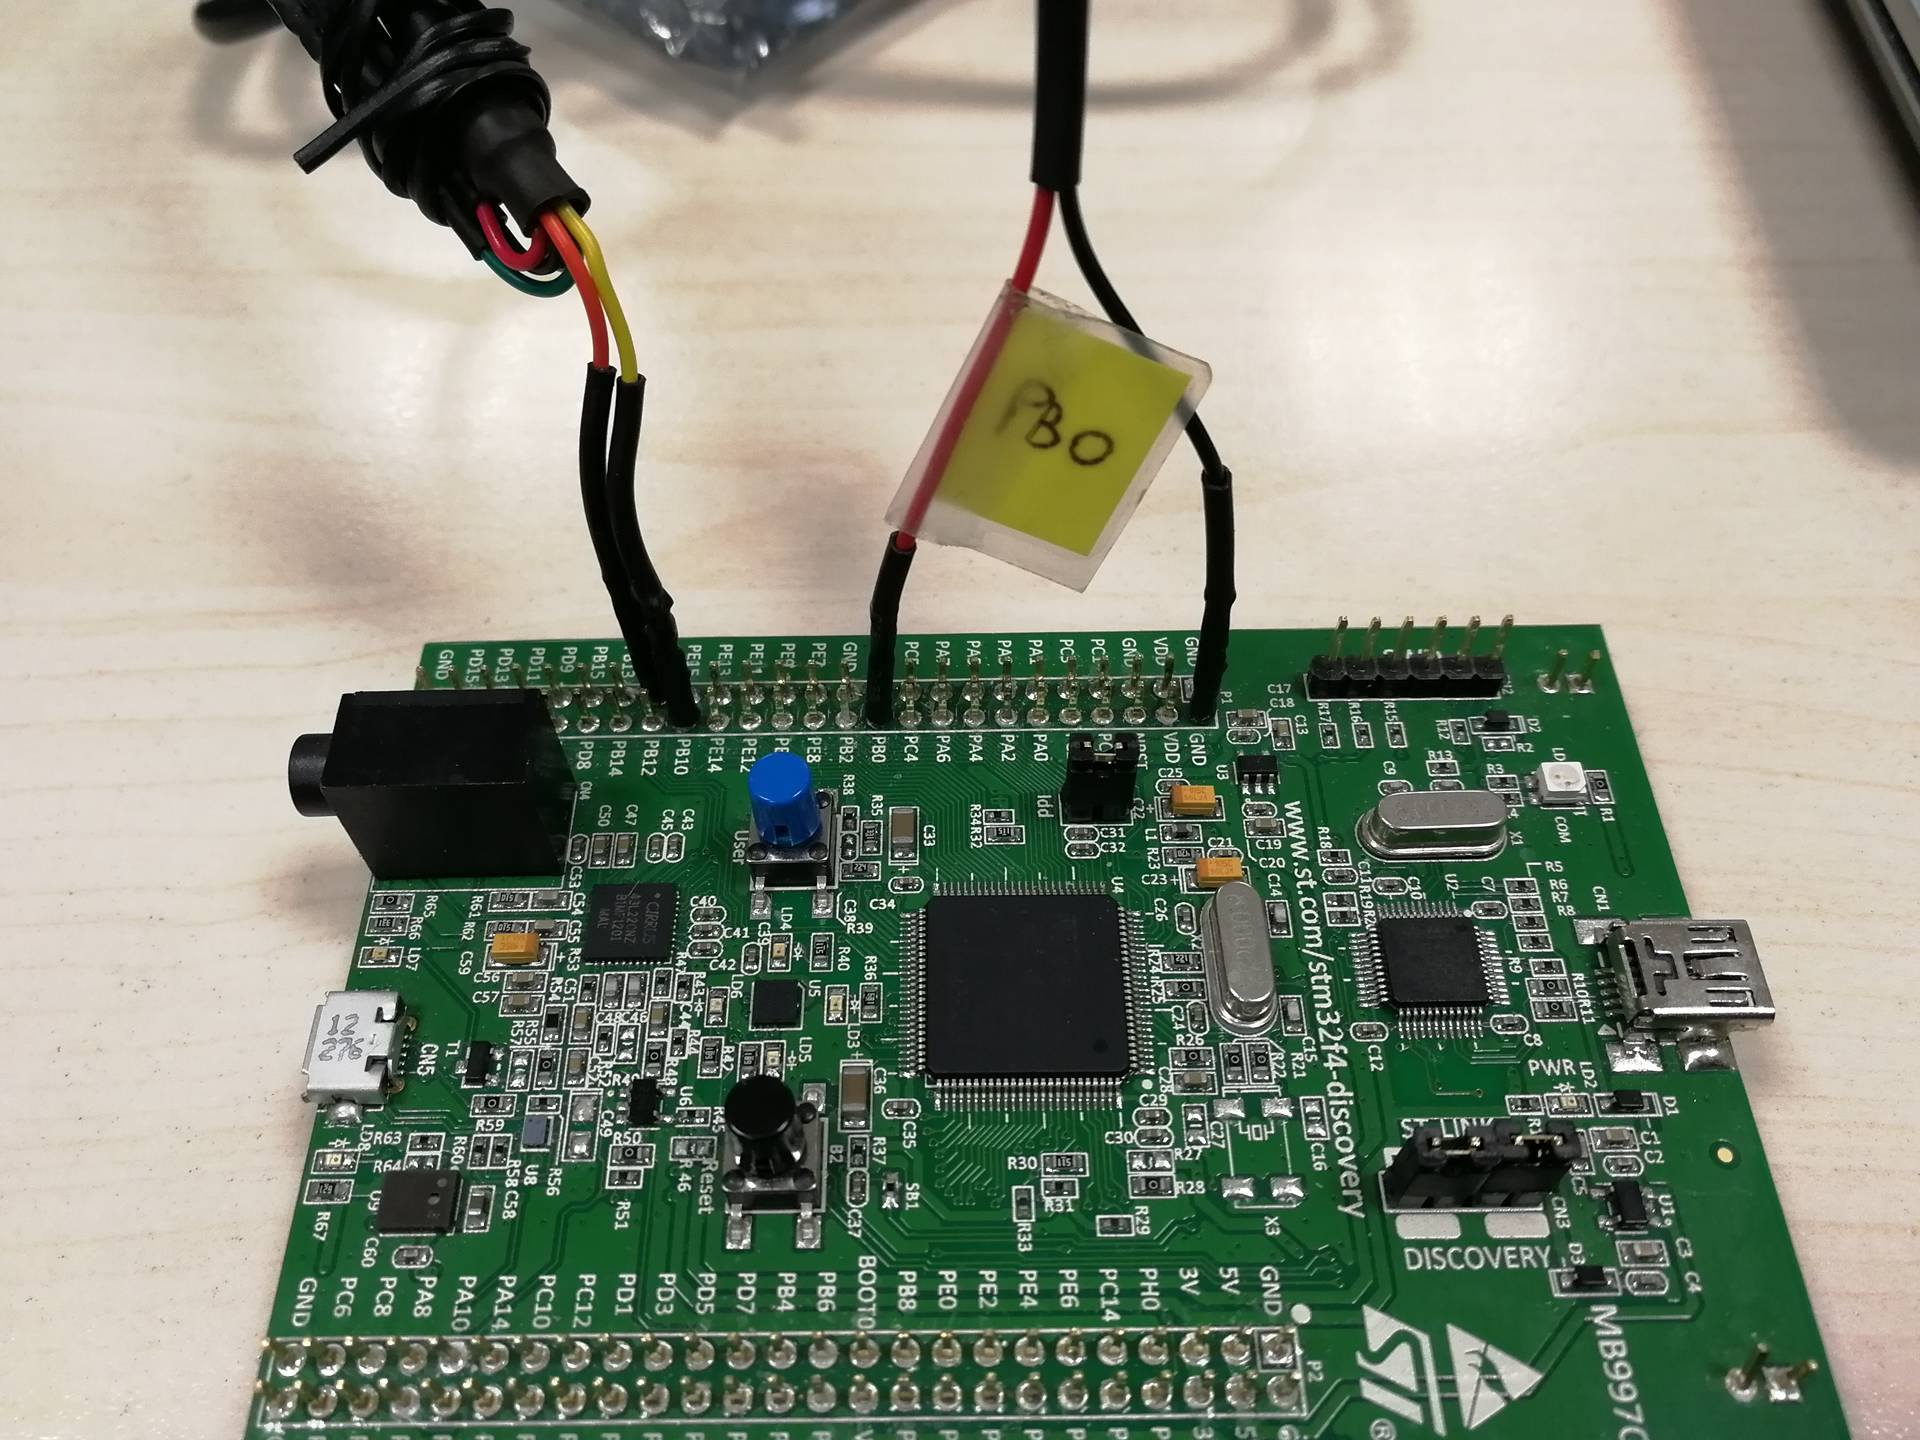
\includegraphics[width=1\textwidth]{./figures/connections.jpg}
  \caption{Connections}
  \label{fig:connections}
\end{figure}

\section{Experimental evaluation}\label{Results}
\subsection{Experimental setup}
\subsection{Results}



\section{Conclusions}

